\let\negmedspace\undefined
\let\negthickspace\undefined
\documentclass[journal]{IEEEtran}
\usepackage[a5paper, margin=10mm, onecolumn]{geometry}
\usepackage{lmodern} % Ensure lmodern is loaded for pdflatex
\usepackage{tfrupee} % Include tfrupee package

\setlength{\headheight}{1cm} % Set the height of the header box
\setlength{\headsep}{0mm}     % Set the distance between the header box and the top of the text

\usepackage{gvv-book}
\usepackage{gvv}
\usepackage{cite}
\usepackage{amsmath,amssymb,amsfonts,amsthm}
\usepackage{algorithmic}
\usepackage{graphicx}
\usepackage{textcomp}
\usepackage{xcolor}
\usepackage{txfonts}
\usepackage{listings}
\usepackage{enumitem}
\usepackage{mathtools}
\usepackage{gensymb}
\usepackage{comment}
\usepackage[breaklinks=true]{hyperref}
\usepackage{tkz-euclide} 
\usepackage{listings}
\usepackage{gvv}                                        
\def\inputGnumericTable{}                                 
\usepackage[latin1]{inputenc}                                
\usepackage{color}                                            
\usepackage{array}                                            
\usepackage{longtable}                                       
\usepackage{calc}                                             
\usepackage{multirow}                                         
\usepackage{hhline}                                           
\usepackage{ifthen}                                           
\usepackage{lscape}
\begin{document}

\bibliographystyle{IEEEtran}
\vspace{3cm}

\title{12.8.3.11}
\author{EE24BTECH11024 - G. Abhimanyu Koushik}
% \maketitle
% \newpage
% \bigskip
{\let\newpage\relax\maketitle}
\textbf{Question:}
Using the method of integration find the area bounded by the curve $\abs{x} + \abs{y} = 1$
\solution\newline
Theoretical Solution:\newline
The curve $\abs{x} + \abs{y} = 1$ consists of 4 lines
\begin{align}
	x+y&=1\\
	-x+y&=1\\
	x-y&=1\\
	-x-y&=1
\end{align}
These lines intersect at points \brak{1,0}, \brak{-1,0}, \brak{0,1} and \brak{0,-1} forming a square. To find the area we can integrate $x+y=1$ from $x=0$ to $x=1$ and then multiply the area by 4 to get the total area   
\begin{align}
	A_0 &= \int_{0}^{1}\brak{1-x}dx\\
	A_0 &= \brak{x-\frac{x^2}{2}}\Big|_0^1\\
	A_0 &= \frac{1}{2}\\
	A &= 4A_0\\
	A &= 2
\end{align}

Computational Solution:\newline

Taking trapezoid shaped strips of small area and adding them all up. Say we have to find the area of $y\brak{x}$ from $x=x_0$ to $x=x_n$, discretize points on the $x$ axis $x_0, x_1, x_2, \dots, x_n$ such that they are equally spaced with step-size $h$. \newline
Sum of all trapezoidal areas is given by,
\begin{align}
  A&=\frac{1}{2}h\brak{y\brak{x_1}+y\brak{x_0}}+ \frac{1}{2}h\brak{y\brak{x_2}+y\brak{x_1}}+\dots+\frac{1}{2}h\brak{y\brak{x_n}+y\brak{x_{n-1}}}\\
  &=h\sbrak{\frac{1}{2}\brak{y\brak{x_0}+y\brak{x_n}}+ y\brak{x_1}+\dots+y\brak{x_{n-1}}}
\end{align}
Let $A\brak{x_n}$ be the area enclosed by the curve $y\brak{x}$ from $x=x_0$ to $x=x_n$, $\brak{x_0, x_1, \dots x_n}$ be equidistant points with step-size $h$.
\begin{align}
  A\brak{x_n+h}=A\brak{x_n}+\frac{1}{2}h\brak{y\brak{x_n+h}+y\brak{x_n}}
\end{align}
We can repeat this till we get required area.\newline
Discretizing the steps, making $A\brak{x_n}=A_n, y\brak{x_n}=y_n$ we get,
\begin{align}
 A_{n+1}=A_n+\frac{1}{2}h\brak{y_{n+1}+y_n}
\end{align}
We can write $y_{n+1}$ in terms of $y_n$ using first principle of derivative. $y_{n+1}=y_n+hy^{\prime}_n$
\begin{align}
  A_{n+1}&=A_n+\frac{1}{2}h\brak{\brak{y_{n}+hy^{\prime}_n}+y_n}\\
  A_{n+1}&=A_n+\frac{1}{2}h\brak{2y_n+hy^{\prime}_n}\\
  A_{n+1}&=A_n+hy_n+\frac{1}{2}h^2y^{\prime}_n\\
  x_{n+1}&=x_n+h
\end{align}

In the given question, $y_n=1 - x_n$ and $y^{\prime}_n=-1$\newline
General Difference Equation will be given by,
\begin{align}
  A_{n+1}&=A_n+hy_n+\frac{1}{2}h^2y^{\prime}_n\\
  A_{n+1}&=A_n+h\brak{1-x_n}+\frac{1}{2}h^2\brak{-1}\\
  A_{n+1}&=A_n -hx_n+\brak{h-\frac{h^2}{2}}\\
  x_{n+1}&=x_n+h
\end{align}
Iterating till we reach $x_n=1$ will return required area. Note, Area obtained is to be multiplied by $4$ as the calculated area only accounts for one quater of the graph.\newline
\begin{figure}[h!]
   \centering
   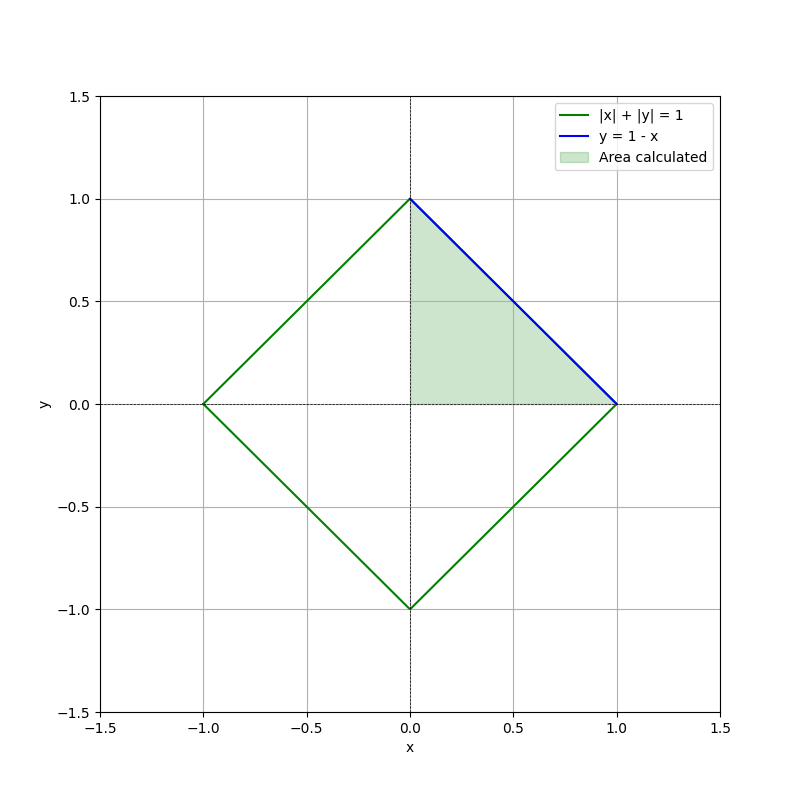
\includegraphics[width=1\columnwidth]{figs/fig.png}
   \caption{Graph of the parabola $\abs{x}+\abs{y} = 1$ and $x+y=1$ and the area of which the integral is calculated}
   \label{stemplot}
\end{figure}
\end{document}
